
% VLDB template version of 2020-08-03 enhances the ACM template, version 1.7.0:
% https://www.acm.org/publications/proceedings-template
% The ACM Latex guide provides further information about the ACM template

\documentclass[sigconf, nonacm]{acmart}

\usepackage{float}

%% The following content must be adapted for the final version
% paper-specific
\newcommand\vldbdoi{XX.XX/XXX.XX}
\newcommand\vldbpages{XXX-XXX}
% issue-specific
\newcommand\vldbvolume{14}
\newcommand\vldbissue{1}
\newcommand\vldbyear{2020}
% should be fine as it is
\newcommand\vldbauthors{\authors}
\newcommand\vldbtitle{\shorttitle} 
% leave empty if no availability url should be set
\newcommand\vldbavailabilityurl{URL_TO_YOUR_ARTIFACTS}
% whether page numbers should be shown or not, use 'plain' for review versions, 'empty' for camera ready
\newcommand\vldbpagestyle{plain} 

\begin{document}
\title{ArgMax in Sliding-Window Aggregation}

%%
%% The "author" command and its associated commands are used to define the authors and their affiliations.
\author{Julian Muders}
\affiliation{%
  \institution{Humboldt-Universität zu Berlin}
  \city{Berlin}
  \country{Germany}
}
\email{mudersju@informatik.hu-berlin.de}

\author{Richard Herrmann}
\affiliation{%
  \institution{Humboldt-Universität zu Berlin}
  \city{Berlin}
  \country{Germany}
}
\email{herrmari@informatik.hu-berlin.de}

\author{Philipp Harnisch}
\affiliation{%
  \institution{Humboldt-Universität zu Berlin}
  \city{Berlin}
  \country{Germany}
}
\email{harnisph@informatik.hu-berlin.de}

%%
%% The abstract is a short summary of the work to be presented in the
%% article.
\begin{abstract}
We wanted to compare the general results for operators of the Reactive Aggregator approach from the original paper~\cite{GeneralIncremental15}
with our own implementation, solely focussing on the ArgMax operator. Our main findings are that \ldots (see \autoref{obtained_results}).
\end{abstract}

\maketitle

%%% do not modify the following VLDB block %%
%%% VLDB block start %%%
\pagestyle{\vldbpagestyle}
\begingroup\small\noindent\raggedright\textbf{PVLDB Reference Format:}\\
\vldbauthors. \vldbtitle. PVLDB, \vldbvolume(\vldbissue): \vldbpages, \vldbyear.\\
\href{https://doi.org/\vldbdoi}{doi:\vldbdoi}
\endgroup
\begingroup
\renewcommand\thefootnote{}\footnote{\noindent
This work is licensed under the Creative Commons BY-NC-ND 4.0 International License. Visit \url{https://creativecommons.org/licenses/by-nc-nd/4.0/} to view a copy of this license. For any use beyond those covered by this license, obtain permission by emailing \href{mailto:info@vldb.org}{info@vldb.org}. Copyright is held by the owner/author(s). Publication rights licensed to the VLDB Endowment. \\
\raggedright Proceedings of the VLDB Endowment, Vol. \vldbvolume, No. \vldbissue\ %
ISSN 2150-8097. \\
\href{https://doi.org/\vldbdoi}{doi:\vldbdoi} \\
}\addtocounter{footnote}{-1}\endgroup
%%% VLDB block end %%%

%%% do not modify the following VLDB block %%
%%% VLDB block start %%%
\ifdefempty{\vldbavailabilityurl}{}{
\vspace{.3cm}
\begingroup\small\noindent\raggedright\textbf{PVLDB Artifact Availability:}\\
The source code, data, and all figures have been made available at \url{https://github.com/muderjul/event_processing_2021}.
\endgroup
}
%%% VLDB block end %%%

\section{Goal and Structure}
\label{goal_and_structure}

The goal of this work was to reconstruct some of the work of~\cite{GeneralIncremental15}, using their conecpt of a so-called Reactive Aggregator. More specifically, we wanted to develop a simple streaming aggregator for the ArgMax operator, based on that approach. Despite limiting our work to a bare minimum at the implementation level, we wanted to compare the results of the paper with the results that we get from our experiments.

Thus, our implementation is oriented after the original implementation architecture (see \autoref{fig:original_architecture}) which contains four main components:
\begin{description}
	\item[Windowing library:] processes the incoming data stream and informs the Reactive Aggregator about inserts, evicts or triggers (updates)
	\item[Reactive Aggregator:] handles the overall flow of the application, receiving events from the windowing library and pushing them to the FlatFAT object
	\item[FlatFAT:] contains all the intermediate results for the aggregation in a tree data structure, using the aggregation operations
	\item[Aggregation operations:] defining the neccessary implementation of the three functions lift, combine and lower for each specific aggregation operation (we only focus on the ArgMax aggregation operation)
\end{description}

\begin{figure}[H]
	\centering
	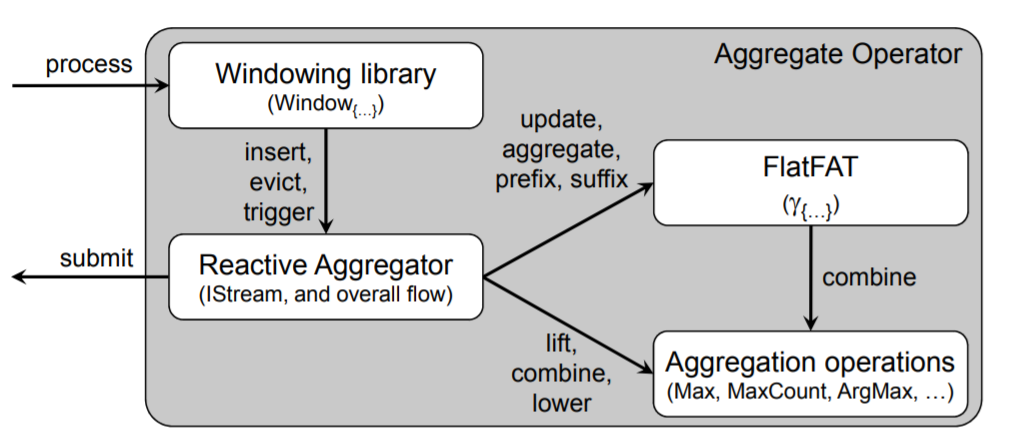
\includegraphics[width=\linewidth]{figures/original_architecture}
	\caption{Overview of the approach published in~\cite{GeneralIncremental15}}
	\label{fig:original_architecture}
\end{figure}

\section{Applied Method}
\label{applied_methods}

\ldots

\section{Obtained Results}
\label{obtained_results}

\ldots

\section{Discussion}
\label{discussion}

\ldots

%%%%%%%%%%%%%%%%%%%%%%%%%%%%%%%%%%%%%%%%%%%%%%
% example of figure and ref from the template:
%\autoref{fig:duck}.
%\begin{figure}
%  \centering
%  \includegraphics[width=\linewidth]{figures/duck}
%  \caption{An illustration of a Mallard Duck. Picture from Mabel Osgood Wright, \textit{Birdcraft}, published 1897.}
%  \label{fig:duck}
%\end{figure}
%%%%%%%%%%%%%%%%%%%%%%%%%%%%%%%%%%%%%%%%%%%%%%

%%%%%%%%%%%%%%%%%%%%%%%%%%%%%%%%%%%%%%%%%%%%%%
% example of double column table from the template:
%\begin{table*}[t]
%  \caption{A double column table.}
%  \label{tab:commands}
%  \begin{tabular}{ccl}
%    \toprule
%    A Wide Command Column & A Random Number & Comments\\
%    \midrule
%    \verb|\tabular| & 100& The content of a table \\
%    \verb|\table|  & 300 & For floating tables within a single column\\
%    \verb|\table*| & 400 & For wider floating tables that span two columns\\
%    \bottomrule
%  \end{tabular}
%\end{table*}
%%%%%%%%%%%%%%%%%%%%%%%%%%%%%%%%%%%%%%%%%%%%%%

%%%%%%%%%%%%%%%%%%%%%%%%%%%%%%%%%%%%%%%%%%%%%%
% example of normal table from the template:
%\begin{table}[hb]% h asks to places the floating element [h]ere.
%  \caption{Frequency of Special Characters}
%  \label{tab:freq}
%  \begin{tabular}{ccl}
%    \toprule
%    Non-English or Math & Frequency & Comments\\
%    \midrule
%    \O & 1 in 1000& For Swedish names\\
%    $\pi$ & 1 in 5 & Common in math\\
%    \$ & 4 in 5 & Used in business\\
%    $\Psi^2_1$ & 1 in 40\,000 & Unexplained usage\\
%  \bottomrule
%\end{tabular}
%\end{table}
%%%%%%%%%%%%%%%%%%%%%%%%%%%%%%%%%%%%%%%%%%%%%%

%\begin{acks}
% This work was supported by the [...] Research Fund of [...] (Number [...]). Additional funding was provided by [...] and [...]. We also thank [...] for contributing [...].
%\end{acks}

%\clearpage

\bibliographystyle{ACM-Reference-Format}
\bibliography{sample}

\end{document}
\endinput
